\documentclass[c_worksheet.tex]{subfiles}


\begin{document}


\chapter{Funktionen}


\section{Warum man Funktionen benutzt} 

Manchmal hat man ein Stück Code geschrieben und möchte es an mehreren Stellen verwenden. Dann kann man das ganze natürlich mehrfach schreiben, aber sinnvoller ist es eine Funktion zu verwenden.

Solche Funktionen kann amn dann einfach aufrufen, selbst wenn man nicht genau weiß, was genau diese Funktion eigentlich tut. So ein bisschen wie eine kleine magische Wolke.

\begin{figure}[h]
\center
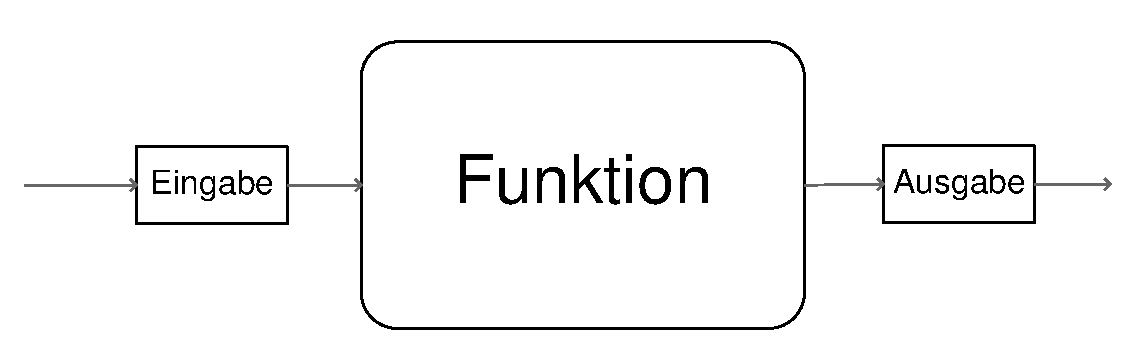
\includegraphics[width=0.9\textwidth]{Grafiken/Funktionen/function}
\end{figure}

Einige solcher Funktionen sind wahrscheinlich bereits bekannt und wurden oft benutzt. So z.B. \textbf{printf} und \textbf{scanf}. \textbf{printf} nimmt als Eingabe einen \emph{String} und liefert als Ausgabe eine Ausgabe auf der Konsole.

Solche Funktionen kann man sich auch selbst definieren. Das allgemeine Schema dazu sieht wie folgt aus:

\begin{lstlisting}[language=c]
<Rueckgabetyp> <name>(<Typ> <p1Name>, .. , <Typ> <pnName>){
	<FunktionsCode>
}
\end{lstlisting}

Der \emph{Rückgabetyp} bezeichnet dabei den Typ des Wertes, den die Funktion am Ende zurück gibt. Also so etwas wie \emph{int}, \emph{float} oder auch \emph{char}. Möchte man nichts zurück geben, ist der \emph{Rückgabetyp} \textbf{void}.

Mit dem \emph{Funktionsnamen} kann man die Funktion später aufrufen.

Mit den \emph{Parametern} kann man der Funktion Werte übergeben. Jedem von ihnen wird ein \emph{Typ} und ein \emph{Parametername} zugeordnet. Mit diesem \emph{Parametername} kann man in der Funktion auf diese Variable zugreifen.

Mit dem Befehl \emph{return} beendet man die Funktion und gibt den Wert zurück, den man zusammen mit dem \emph{return} Befehl angibt, zurück.

\section{Sicht aus der Mathematik}

Funktionen kennt man bereits zu genüge aus der Mathematik und im Prinzip sind Funktionen in \textbf{C} genau das selbe. Sie haben eine Eingabe, eine Ausgabe und dazwischen machen sie die unterschiedlichsten Dinge.

Zum Beispiel die normale Lineare Funktion die man aus der Mathe kennt:

\begin{align*}
 f(x) &= m*x + b
 \end{align*} 

 Diese kann man quasi genau so auch in \textbf{C} schreiben. Dafür nehmen wir \(m=2\) und \(b=1\) an.

\lstinputlisting{CodeSnippets/Funktionen/linear_function.c} 


\section{Rückgabe} 

Mit dem \textbf{return} Keyword, beendet man immer die Funktion, in der sich selbiges befindet. Deswegen beendet man auch das Hauptprogramm mit dem \textbf{return 0} am Ende der \emph{main} Funktion.

\lstinputlisting{CodeSnippets/Funktionen/return.c}

Mit dem \textbf{return}	Keyword liefert man den Wert dahinter ``zurück nach oben''. Im Prinzip kann man sich das so vorstellen, dass die Funktion diesen Wert annimmt, wenn man sie in eine Gleichung schreibt.

\lstinputlisting{CodeSnippets/Funktionen/return2.c}  


\section{Funktionsaufruf} 

Funktionen können ganz einfach über ihren Namen aus der \emph{main} Methode heraus aufgerufen werden.

\lstinputlisting[firstline=1, lastline=3]{CodeSnippets/Funktionen/addition.c} 

Die Funktion hat den namen ``addition'', gibt einen Wert vom Typ \textbf{int} zurück, bekommt 2 Parameter vom Typ \emph{int} mit dem Namen \(a\) und \(b\) und berechnet deren Summe. Diese wird mit dem \emph{return} Befehl zurück gegeben.\\
Die Funktion kann dann ganz einfach in der \emph{main} Funktion aufgerufen werden.

\lstinputlisting[firstline=5, lastline=21]{CodeSnippets/Funktionen/addition.c} 

Mit den \emph{Parameternamen} kann innerhalb der Funktion auf diese zugegriffen werden. Wichtig dabei ist, dass diese Parameter nur in der Funktion selbst sichtbar (das heißt benutzbar) sind.



\section{Sichtbarkeiten} 

Alle Variablen die innerhalb einer Funktion \emph{initialisiert} werden, sind nur dort sichtbar und verwendbar. Es kann durchaus mehrere Variablen mit gleichem Namen geben.

\lstinputlisting{CodeSnippets/Funktionen/sichtbarkeit.c} 

 Eine Funktion erzeugt immer eine \textbf{lokale Kopie} der Parameter. Wie im vorangehen Beispiel gesehen, wird das \(y\) aus der \emph{main} Methode nicht verändert, obwohl man es der dummy Funktion übergibt. Diese erzeugt aber ihre eigene Kopie davon und arbeitet nur auf dieser. \\

 Wichtig ist auch, dass Namen doppelt vorkommen können. Folgendes Beispiel behandelt einen Fall, der am Anfang sehr verwirrend ist.

 \lstinputlisting{CodeSnippets/Funktionen/same_name.c} 

Die Variable die wir an die square Funktion übergeben, könnte jeden erdenklichen Namen haben, es ist reiner Zufall, dass sie den selben Namen, wie der Funktionsparameter hat.



\section{Beispiele}

Funktionen müssen weder Parameter, noch etwas zurück geben, wie folgendes Beispiel zeigt.

\lstinputlisting{CodeSnippets/Funktionen/foo.c}  

Funktionen können beliebig komplex werden. Folgende Funktion berechnet zum Beispiel die Fakultät einer Zahl.

\lstinputlisting{CodeSnippets/Funktionen/fakultaet.c} 



\section{Rekursion}

Unter \emph{Rekursion} versteht man, dass sich eine Funktion \textbf{selbst} wieder aufruft. Am besten wird dies an Beispielen klar

\lstinputlisting{CodeSnippets/Funktionen/recursion.c}

Auch die GaußSumme lässt sich rekursiv berechnen. Man beachte, dass der rekursive Aufruf hier mit einem \textbf{return} Befehl geschieht. Wenn die Rekursion ``ganz unten'' angelangt ist, wird sie einen Wert annehmen und diesen ``nach oben zurück reichen''.


\lstinputlisting{CodeSnippets/Funktionen/recursive_sum.c} 



\end{document}